\section{Design and Implementation}
The development of the web application went through a lot of ideas before settling on the current choice of technologies used. The application uses the JavaScript library React for the frontend and user interface, and the Python web framework Flask for the backend algorithms. The initial designs, choices made and features implemented are expanded on below.

\subsection{Software Requirements}
Before any software was written, a list of requirements for the software was made. These are features that the software must have in order to fulfill the relevant objectives, and were subsequently tested throughout the development of the web application:
\begin{enumerate}
    \item Allow a user to enter Dyck words.
    \item Validate a given input and provide a relevant error message if required.
    \item Display the given Dyck word with the ability for manual interaction via a mouse.
    \item Verify that the characters selected are a valid move before allowing them to be paired.
    \item Allow for the use of strategies from literature (Simple, Non-Simple recursive), as well as our own strategies (Simple Greedy, Brute Force).
    \item If selecting a strategy, generate a list of moves before visualising the play.
    \item Display the list of moves, and allow the user to jump to any move in the play.
    \item Display a running width counter from the moves seen so far, and the width of the overall play if a strategy has been used.
    \item (OPTIONAL) Allow for a mix between manual re-pairing and the use of pre-defined strategies (e.g. re-pairing the first half of a word using a strategy, and completing the second half using manual selections).
    \item Allow the user to brute force a given list of Dyck Words, and return the optimal widths of each along with the re-pairing.
\end{enumerate}

\subsection{Initial Design}

The project was initially to be a local Python only application, using Tkinter. This was because the author is most familiar with the Python programming language, and has some limited experience with the Tkinter library. However, early prototypes of this software using Tkinter proved to be cumbersome to work with and have a dated visual style. Alternative Python UI libraries, such as PyQt and Kivy, were also considered, but proved to have learning curves no steeper than using an entirely different language.
\begin{figure}[H]
    \centering
    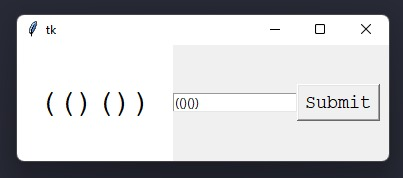
\includegraphics[scale = 0.7]{./images/tkinter-gui.jpeg}
    \caption{An early iteration of the software using Tkinter}
\end{figure}
\noindent We then turned our attention to the prospect of a web application; the author again had some limited experience with HTML/CSS but using these languages to control the layout and sizing of the UI seemed much more intuitive. This approach also naturally allowed for separation between the UI and the strategies, and the author's familiarity with Python could still be leveraged. The author had also wished to learn the technologies used for web development, so this seemed like the natural approach to take.


\par\null\par
\noindent If a web-application was to be used, some way of communicating between the code for the UI and Python was needed. This led to considering React, which is a JavaScript library used to create user interfaces \cite{whatisReact}.

\par\null\par
\noindent A second prototype was then created to confirm this was indeed the right choice. This seemed promising; the implementation was not overly complicated, and the layout was easy to control. 